\section{Opportunities for advanced control}

\subsection{Model Predictive Control}
\subsubsection{Introduction}
Model Predictive control is an advanced control technique that can cope with complex multivariate control problems. A model predictive controller (MPC) functions by taking in current measurements of manipulated variables (MVs) and disturbances (DVs) from the plant and then calculates the future profile for the controlled variables (CVs) and constraint variables in order to predict the optimal values for the manipulated variables. The controller performs two sets of calculations, first to determine the future profile of CVs ('set-point calculations'), and second the optimal values for MVs ('control calculations') to reach the desired set-points. 

The future profile of CVs are calculated from solving an optimisation problem that determines the set points for the CVs for a period of time in the future ('prediction horizon'). The objective function for this optimisation is usually to maximise profit or minimise cost, and is subject to inequality constraints that can vary with time such as variations in process conditions, functional instrumentation and economic data such as pricing. These set-points are re-calculated each time new data is received. The optimal values for MVs are then calculated. Unlike traditional PID controllers, a sequence of MV steps are calculated by splitting the prediction horizon into a number of sampling intervals, and the effects on CVs are determined in order to move them closer to the desired set-points (see Figure \ref{fig:MPC}). 

    \begin{wrapfigure}{r}{0.5\linewidth}
        \centering
        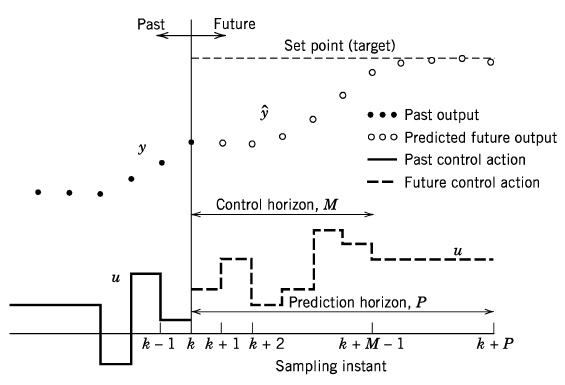
\includegraphics[width=\linewidth]{chapters/4-operation-control/4-Figures/MPC-Seborg-2011.png}
        \caption{Illustration of MPC in action, taken from \textcite{}. $u$ is a manipulated variable, and $y$ is a controlled variable}
        \label{fig:MPC}
    \end{wrapfigure}

The goal of the MPC is to minimise the differences between the set-point and the predicted values of the CV at each sampling instant. Expressing these errors in a vector to the MPC algorithm returns a combination of MV steps that minimises the total error. The MPC then outputs a signal to the actuators to implement the changes to the MVs. However, only the first step is performed. The MPC then receives new measurements from transmitters on the plant, and then re-calculates the trajectory of the CVs with an updated time horizon. In this way the MPC iteratively solves for the optimal MV action to bring the CV closer to its setpoint. 

The accuracy of MPC algorithms depends heavily on the dynamic model of the process it utilises for calculations. Assuming a good dynamic model exists, Model Predictive Control has serveral advantages over PID controllers, namely that it captures interactions between control loops, handles multiple inputs and predict multiple outputs, and takes into consideration physical constraints on actuators. 

\subsubsection{Application to Nitroma's plant}
Nitroma's plant has specialised units such as an intensified shell and tube reactor, melt crystalliser and hydraulic wash column. Although detailed designs of these units have been provided in the relevant report sections, a dynamic model for the entire plant is missing. MPC will only be effective if a good dynamic model can be constructed. 

The most common method for identifying dynamic models is Finite Impulse Reponse (FIR) and Auto Regressive with eXternal inputs (ARX). Step experiments for each MV-CV pair will have to be conducted on Nitroma's plant to measure the dynamic response of each. FIR can then be used to calculate the dead times for each MV-CV pair. This is then used in ARX along with the experimental step data to calculate coefficients relating the mv-cv pairs (see Equation \ref{eq:ARX} for an ARX process model for a single-input, single-output process. $y$ is the CV, $u$ is the MV, $d$ is the dead time, $\nu$, $b$, $a$ are constants). The set of MV-CV equations would constitute a dynamic model for Nitroma's plant. 

\begin{equation} \label{eq:ARX}
    y_k = \sum_{i=1}^{\nu}a_{i}y_{k-i} + \sum_{i=1}^{a}b_{i}u_{k-d-i}
\end{equation}

Once a dynamic model is established, key controlled and manipulated variables will need to be set. While a comprehensive list of CVs and MVs is found in the plant wide survey in \ref{sec:PWS}, a summary table with key information is shown in Table \ref{tab:key-parameters}. A key parameter to control is the feed throughput to reactor R101, as this reactor produces the precursors for all 3 end products and hence affects the production capacity. The  

\begin{table}[h]
\centering
    \caption{Summary of key control parameters across the whole plant}
    \label{tab:key-parameters}
\begin{tabular}{@{}lll@{}}
\toprule
\textbf{Key control variables (CVs)}        & \textbf{Key manipulated variables (MVs)} & \textbf{Key disturbances} \\ \midrule
Temperatures in reactors and crystallisers  & Utility flowrates                        & Utility flowrates         \\
Feed rate to reactor R101                   & Feed flowrates                           & Utility temperatures      \\
Feed ratio to reactor R101                  & Outlet flowrates from units              & Feed quality              \\
Compositions of the 3 product streams       & Electrical input to electrical heaters   & Recycle flowrates         \\
Inventory controls (pressure, liquid level) &                                          & Ambient temperature       \\ \bottomrule
\end{tabular}
\end{table}



\subsection{Real-time control}